% !TEX root = ../../../main.tex

\toggletrue{image}
\togglefalse{imagehover}
\chapterimage{fred_2007-06-25_modified}
\chapterimagetitle{\uppercase{Ideen}}
\chapterimageurl{fonflatter.de/2007/06/25/644-ideen/}

%\pdfgentounicode=0

\chapter{Geheimschriften}
\label{chapter-geheimschriften}

Mit der Entdeckung der Schriften wurden erstmals schriftliche Nachrichten ausgetauscht. Nicht immer sollte jeder diese Nachrichten lesen dürfen.  Die einfachste Möglichkeit, den Inhalt einer Nachricht nicht direkt lesbar zu machen, ist die Vereinbarung einer \say{geheimen Sprache}. Wir bezeichnen diese als \textbf{Geheimschriften}. Die Lernziele lauten:


\newcommand{\geheimschriftenLernziele}{
\protect\begin{todolist}
\item Sie erklären das Kommunikationsszenario für Geheimschriften.
\item Sie wenden die Geheimschrift \texttt{POLYBIOS} an.
\item Sie wenden die Geheimschrift \texttt{FREIMAURER} an.
\item Sie diskutieren die Sicherheit von Geheimschriften. 
\end{todolist}
}

\lernziel{\autoref{chapter-geheimschriften}, \nameref{chapter-geheimschriften}}{\protect\geheimschriftenLernziele}

\geheimschriftenLernziele


\section{Kommunikationsszenario}

\autoref{figure-kommunikationsszenario-geheimschriften} konkretisiert die Kommunikation und zeigt die Fachbegriffe für Geheimschriften.

\begin{figure}[htb]
\centering
\begin{tikzpicture}
\node [cloud, draw, cloud puffs=7, cloud puff arc=120, aspect=3, text width=2.5cm, align=center] (medium) at (0,0) {\footnotesize Übertragungsmedium};

\node[inner sep=0pt] (alice) at (-6,2)
    {
\includegraphics[scale=0.25]{alice_tiny}};
\node[text width=2cm, align=center] (sender) at (-5, 2) {Sender (Alice)};
\node[rectangle, fill=black!25] (chiff) at (-5.5, 0) {Chiffrierung};
\draw[-latex, very thick] (-5.5, 1.5) -- (chiff.north) node[left, midway] {Klartext};
\draw[-latex, very thick] (chiff.east) -- (medium.west) node[above, midway] {Geheimtext};

\node[inner sep=0pt] (bob) at (5,2)
    {
\includegraphics[scale=0.25]{bob_tiny}};
\node[text width=2cm, align=left] (empfaenger) at (6.5, 2) {Empfänger (Bob)};
\node[rectangle, fill=black!25] (dechiff) at (5.5, 0) {Dechiffrierung};
\draw[-latex, very thick] (dechiff.north) -- (5.5, 1.5) node[right, midway] {Klartext};
\draw[-latex, very thick] (medium.east) -- (dechiff.west) node[above, midway] {Geheimtext};

\node[inner sep=0pt] (eve) at (-0.75,-2.5)
    {
\includegraphics[scale=0.25]{eve_tiny}};
\node[text width=3cm, align=center] (pangreifer) at (0.75, -2.5) {Passiver Angreifer (Eve)};
\draw[-latex, very thick] (medium.south) -- (0, -2) node[right, midway] {Geheimtext (Kopie)};

\end{tikzpicture}
\caption{Kommunikationsszenario bei Geheimschriften.}
\label{figure-kommunikationsszenario-geheimschriften}
\end{figure}

Der Inhalt der Nachricht ist in einer Sprache verfasst, die beide verstehen. Wir bezeichnen diesen Inhalt fortan als \textbf{Klartext}. Die \textbf{Chiffrierung} ist ein Verfahren, das einen gegebenen Klartext in einen \textbf{Geheimtext} umwandelt. Nur der Geheimtext wird übertragen. Die \textbf{Dechiffrierung} wandelt den Geheimtext in den Klartext zurück.

\begin{important}
Nur Alice und Bob kennen das \textbf{Verfahren} zum Chiffrieren bzw. Dechiffrieren. Dies stellt den Wissensvorsprung gegenüber Eve dar.
\end{important}

Klartext und Geheimtext sind jeweils ein \textbf{Wort} über einem Alphabet\footnote{In der Informatik ist ein Alphabet nicht auf Buchstaben beschränkt. Ein Alphabet bezeichnet eine nicht leere Menge von Zeichen.}.

\begin{definition}[Klartextalphabet und Geheimtextalphabet]
Das \textbf{Klartextalphabet} ist das Alphabet für den Klartext. Das \textbf{Geheimtextalphabet} ist das Alphabet für den Geheimtext. Die beiden Alphabet müssen \textbf{nicht} identisch sein und können beliebige \textbf{Zeichen} beinhalten.
\end{definition}

Nur Alice und Bob kennen die Verfahren zur Chiffrierung und Dechiffrierung und müssen dies \textbf{vor} der Kommunikation vereinbaren. Wir zeigen nun zwei konkrete Geheimschriften.

\begin{hinweis}
	Wir können uns den Einsatz einer Geheimschrift wie folgt vorstellen: Wir möchten einem Mitschüler eine Nachricht mit einem Zettel mitteilen\footnote{Dies war vor WhatsApp und Co. eine gängige Praxis im Klassenzimmer.}. Nun kann es vorkommen, dass die Lehrperson den Zettel sieht und \say{abfängt}. Wir möchten jedoch vermeiden, dass die Lehrperson den Inhalt der Nachricht lesen kann. Deshalb vereinbaren wir eine Geheimschrift.
\end{hinweis}

\section{Die Geheimschrift \texttt{POLYBIOS}}

Die Geheimschrift des griechischen Schriftstellers Polybios (sprich Polübios) benutzt \autoref{table-polybios}. Ursprünglich (\num{200} Jahre v. u. Z.) wurde das griechische Alphabet mit \num{24} Zeichen benutzt.

\begin{table}[htb]
\centering
\begin{minipage}{0.3\textwidth}
\centering
\begin{tblr}{
    colspec = {c|[2pt]c|c|c|c|c}
  }
\textbf{}  & \textbf{1} & \textbf{2} & \textbf{3} & \textbf{4} & \textbf{5} \\ \hline[2pt]
\textbf{1} & A          & B          & C          & D          & E          \\ \hline
\textbf{2} & F          & G          & H          & I          & K          \\ \hline
\textbf{3} & L          & M          & N          & O          & P          \\ \hline
\textbf{4} & Q          & R          & S          & T          & U          \\ \hline
\textbf{5} & V          & W          & X          & Y          & Z          \\
\end{tblr}
\caption{Das J wurde zur Vereinfachung weggelassen.}
\label{table-polybios}
\end{minipage}
\hfill
\begin{minipage}{0.3\textwidth}
\centering
\begin{tblr}{
    colspec = {c|[2pt]c|c|c|c|c},
    cell{1}{6} = {orange!25},
    cell{4}{1} = {blue!25},
    cell{1}{1} = {white},
    cell{4}{6} = {green!25}
  }
\textbf{}  & \textbf{1} & \textbf{2} & \textbf{3} & \textbf{4} & \textbf{5} \\ \hline[2pt]
\textbf{1} & A          & B          & C          & D          & E          \\ \hline
\textbf{2} & F          & G          & H          & I          & K          \\ \hline
\textbf{3} & L          & M          & N          & O          & P          \\ \hline
\textbf{4} & Q          & R          & S          & T          & U          \\ \hline
\textbf{5} & V          & W          & X          & Y          & Z          \\
\end{tblr}
\caption{Der Buchstabe P wird zu \num{35} chiffriert.}
\label{table-polybios-cipher}
\end{minipage}
\hfill
\begin{minipage}{0.3\textwidth}
\centering
\begin{tblr}{
    colspec = {c|[2pt]c|c|c|c|c},
    row{4} = {blue!25},
    column{3} = {orange!25},
    cell{4}{3} = {green!25}
  }
\textbf{}  & \textbf{1} & \textbf{2} & \textbf{3} & \textbf{4} & \textbf{5} \\ \hline[2pt]
\textbf{1} & A          & B          & C          & D          & E          \\ \hline
\textbf{2} & F          & G          & H          & I          & K          \\ \hline
\textbf{3} & L          & M          & N          & O          & P          \\ \hline
\textbf{4} & Q          & R          & S          & T          & U          \\ \hline
\textbf{5} & V          & W          & X          & Y          & Z          \\
\end{tblr}
\caption{Das Ziffernpaar \num{32} wird zu M dechiffriert.}
\label{table-polybios-decipher}
\end{minipage}
\end{table}

Die Zeilen und Spalten der \num{5} $\times$ \num{5}-Tabelle sind jeweils mit den Zahlen \num{1} bis \num{5} durchnummeriert. Die Buchstaben des lateinischen Alphabets werden zeilenweise von links nach rechts und von oben nach unten eingetragen. Die Alphabete sind somit:

\begin{itemize}
\item Klartextalphabet: A, B, C, D, E, F, G, H, I, K, L, M, \dots , S, T, U, V, W, X, Y, Z
\item Geheimtextalphabet: 1, 2, 3, 4, 5
\end{itemize}

\subsection{Chiffrieren und Dechiffrieren}

Jeder \textbf{Buchstabe} wird durch ein \textbf{Ziffernpaar} ersetzt. Dazu suchen wir den Buchstaben in \autoref{table-polybios} und chiffrieren diesen durch die Ziffer in der ersten Spalte, gefolgt von der Ziffer in der ersten Zeile. Dies verwenden wir dann, um ganze Wörter zu chiffrieren.

\begin{example}
\autoref{table-polybios-cipher} zeigt ein Beispiel für den Buchstaben P. Das Wort PARTY wird somit zu \num{35}\num{11}\num{42}\num{44}\num{54} chiffriert.
\end{example}

Für die Dechiffrierung teilen wir den Geheimtext in \num{2}er-Gruppen auf. Jede \num{2}er-Gruppe wird einzelnen dechiffriert. Die erste Ziffer der \num{2}er-Gruppe definiert die Zeile, die zweite Ziffer die Spalte. Wir erhalten den Klartextbuchstaben an der Stelle, wo sich Zeile und Spalte kreuzen. 

\begin{example}
\autoref{table-polybios-decipher} zeigt ein Beispiel für den Buchstaben M. Der Geheimtext \num{32}\num{15}\num{33}\num{43}\num{11} wird somit zu MENSA dechiffriert.
\end{example}

\section{Die Geheimschrift \texttt{FREIMAURER}}

Seit dem Mittelalter existieren die Geheimbünde der Freimaurer. Zu Beginn wurde eine Geheimschrift benutzt. \autoref{figure-freimaurer} durfte nur in Sand oder Mehl aufgeschrieben werden und musste dann auswendig gelernt werden.

\begin{figure}[htb]
\centering
\begin{minipage}{0.45\textwidth}
\centering
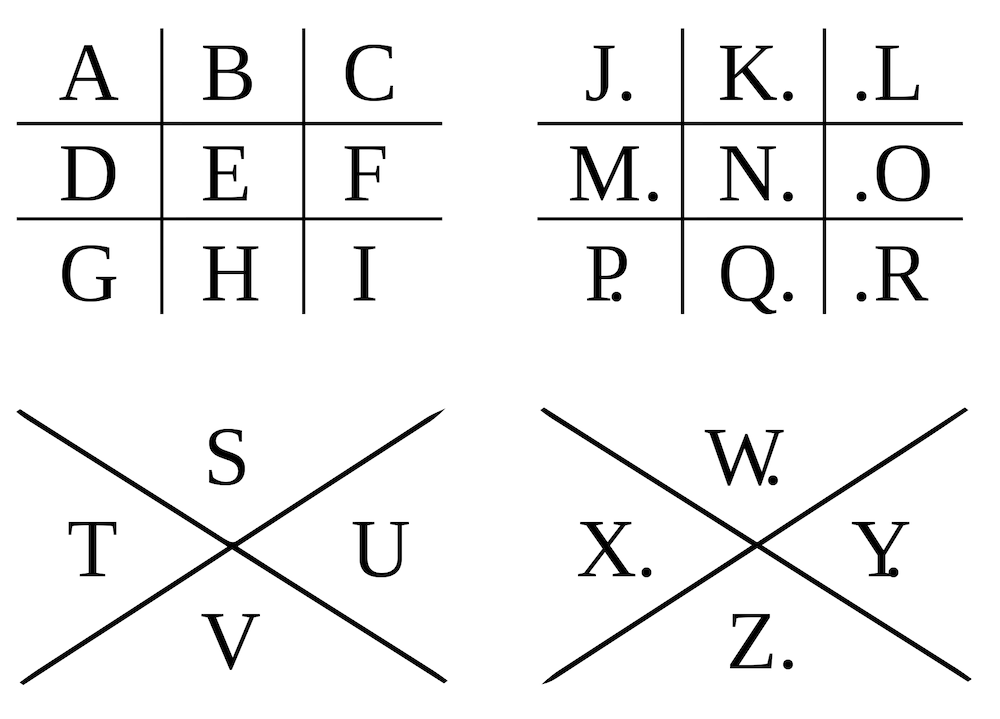
\includegraphics[scale=0.2]{pigpen}
\caption{Freimaurer-Quadrat für \num{26} Buchstaben.}
\label{figure-freimaurer}
\end{minipage}
\hfill
\begin{minipage}{0.45\textwidth}
\centering
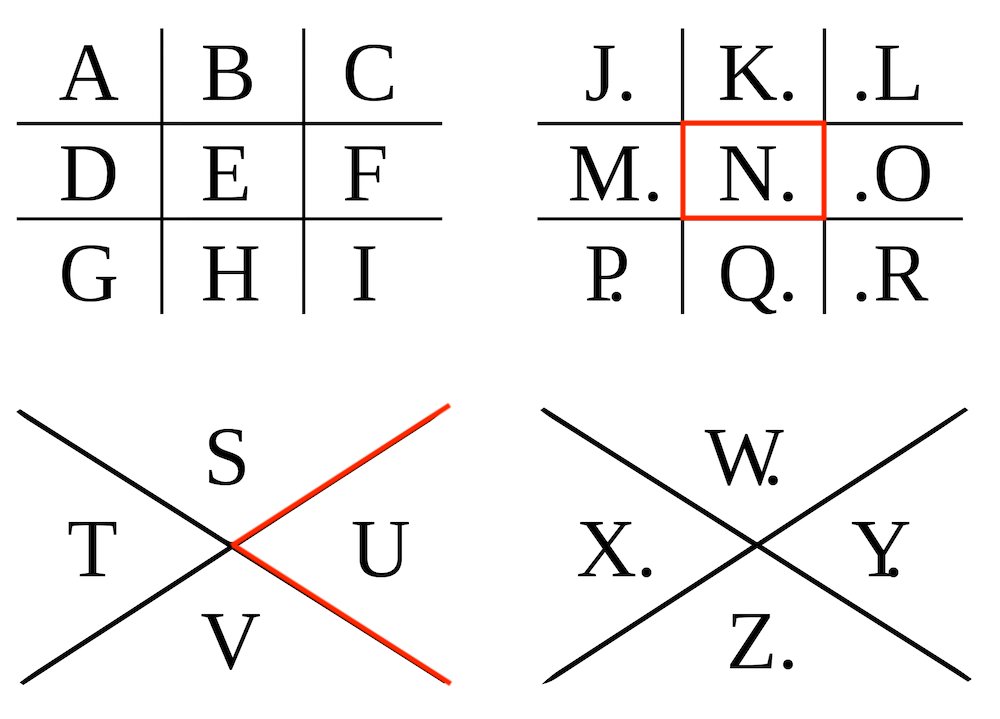
\includegraphics[scale=0.2]{pigpen_examples}
\caption{Das N wird zu {\pigpenfont N} chiffriert, das U zu {\pigpenfont U}.}
\label{figure-freimaurer-beispiel}
\end{minipage}
\end{figure}

Die Alphabete für diese Geheimschrift lauten:

\begin{itemize}
\item Klartextalphabet: A, B, C, D, E, F, G, H, I, K, L, M, \dots , S, T, U, V, W, X, Y, Z
\item Geheimtextalphabet: {\pigpenfont A \pigpenfont B \pigpenfont C \pigpenfont D \pigpenfont E \pigpenfont F \pigpenfont G \pigpenfont H \pigpenfont I \pigpenfont J \pigpenfont K \pigpenfont L \pigpenfont M \pigpenfont N \pigpenfont O \pigpenfont P \pigpenfont Q \pigpenfont R \pigpenfont S \pigpenfont T \pigpenfont U \pigpenfont V \pigpenfont W \pigpenfont X \pigpenfont Y \pigpenfont Z}
\end{itemize}

\subsection{Chiffrieren und Dechiffrieren}

Es wird Buchstabe für Buchstabe aus dem Klartext chiffriert. Dazu suchen wir den Buchstaben im Freimaurer-Quadrat (\autoref{figure-freimaurer}). Der Buchstabe wird dann durch die \textbf{Aussenlinien} und \textbf{gegebenenfalls den Punkt} ersetzt.

\begin{example}
\autoref{figure-freimaurer} zeigt ein Beispiel für die Buchstaben N und U. Das Wort PARTY wird somit zu {\pigpenfont PARTY} chiffriert.
\end{example}

Es wird Zeichen für Zeichen dechiffriert. Wir suchen im Freimaurer-Quadrat (\autoref{figure-freimaurer}) die Linien und gegebenenfalls den Punkt und ersetzen dann das Zeichen durch den darin enthaltenen Buchstaben.

\begin{example}
Mit \autoref{figure-freimaurer} wird {\pigpenfont D} zum Buchstaben D dechiffriert. Der Geheimtext {\pigpenfont MENSA} wird somit zu MENSA dechiffriert.
\end{example}

\section{Sicherheit}
\label{section-geheimschriften-sicherheit}

Die Sicherheit bei Geheimschriften basiert darauf, dass die Verfahren zur Chiffrierung und Dechiffrierung \textbf{geheim} bleiben. Nur Alice und Bob kennen die Verfahren. Keine Geheimschrift kann jedoch lange im Einsatz sein, ohne das Risiko, dass die Verfahren zur gelüftet werden. Ein passiver Angreifer kann dann den Geheimtext leicht lesbar machen.

\begin{definition}[Security by Obscurity]
Wenn die Sicherheit eines Verfahrens allein auf dessen \textbf{Geheimhaltung} basiert, dann sprechen wir von \say{Sicherheit durch Unklarheit} (eng. security by obscurity).
\end{definition}

Geheimschriften folgen diesem Prinzip. Wir müssen typischerweise einen hohen Aufwand betreiben, damit das Geheimnis nicht gelüftet wird. Dies ist für die Praxis ungeeignet und zu unsicher. Deshalb sind Geheimschriften in \ac{IT}-Systemen nicht im Einsatz. Wir benötigen also ein besseres Verfahren für die sichere Kommunikation.

\newpage

\section{Aufgaben}
\label{section-aufgaben-geheimschriften}

\begin{figure}[htb]
\centering
\begin{minipage}{0.45\textwidth}
\centering
\begin{tblr}{
    colspec = {c|[2pt]c|c|c|c|c}
  }
\textbf{}  & \textbf{1} & \textbf{2} & \textbf{3} & \textbf{4} & \textbf{5} \\ \hline[2pt]
\textbf{1} & A          & B          & C          & D          & E          \\ \hline
\textbf{2} & F          & G          & H          & I          & K          \\ \hline
\textbf{3} & L          & M          & N          & O          & P          \\ \hline
\textbf{4} & Q          & R          & S          & T          & U          \\ \hline
\textbf{5} & V          & W          & X          & Y          & Z          \\
\end{tblr}
\caption{\texttt{POLYBIOS}}
\end{minipage}
\hfill
\begin{minipage}{0.45\textwidth}
\centering
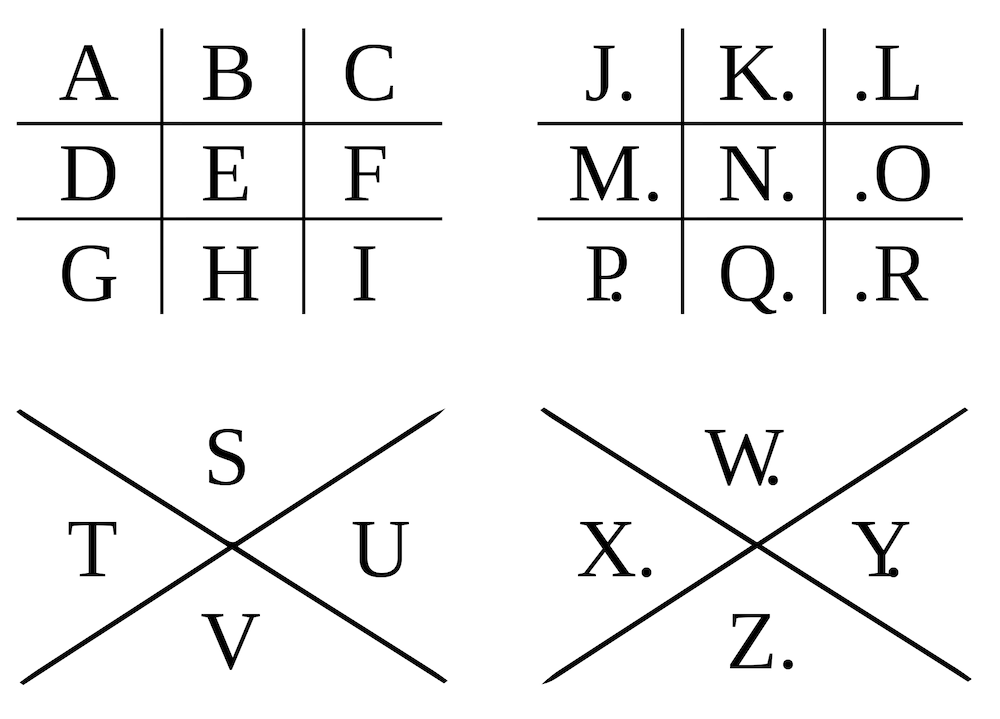
\includegraphics[scale=0.15]{pigpen}
\caption{\texttt{FREIMAURER}}
\end{minipage}
\end{figure}


\begin{enumerate}
\item Chiffrieren Sie LANGBAU mit \texttt{POLYBIOS}.
\fillwithgrid{1in}
\item Dechiffrieren Sie 124215112521114344 13314512 mit \texttt{POLYBIOS}.
\fillwithgrid{1in}
\item Chiffrieren Sie PALAZZO mit \texttt{FREIMAURER}.
\fillwithgrid{1in}
\item Dechiffrieren Sie {\pigpenfont ROLLERCOASTER} mit \texttt{FREIMAURER}.
\fillwithgrid{1in}
\item Lesen Sie \autoref{section-geheimschriften-sicherheit}. Finden Sie ein \say{nicht Informatik-Beispiel} aus dem Alltag, bei dem Sie Security by Obscurity benutzen.
\fillwithgrid{\stretch{1}}
\end{enumerate}